\documentclass[border=10pt]{standalone}

\usepackage{tikz}
\usetikzlibrary{shapes, arrows.meta}

\tikzset{%
  >={Latex[width=2mm,length=2mm]},
  % Specifications for style of nodes:
  base/.style = {
    minimum height=1cm,
    draw=black,
    text centered,
    font=\sffamily
  },
  action/.style={base, rectangle},
  test/.style={base, diamond, aspect=3,},
}

\begin{document}
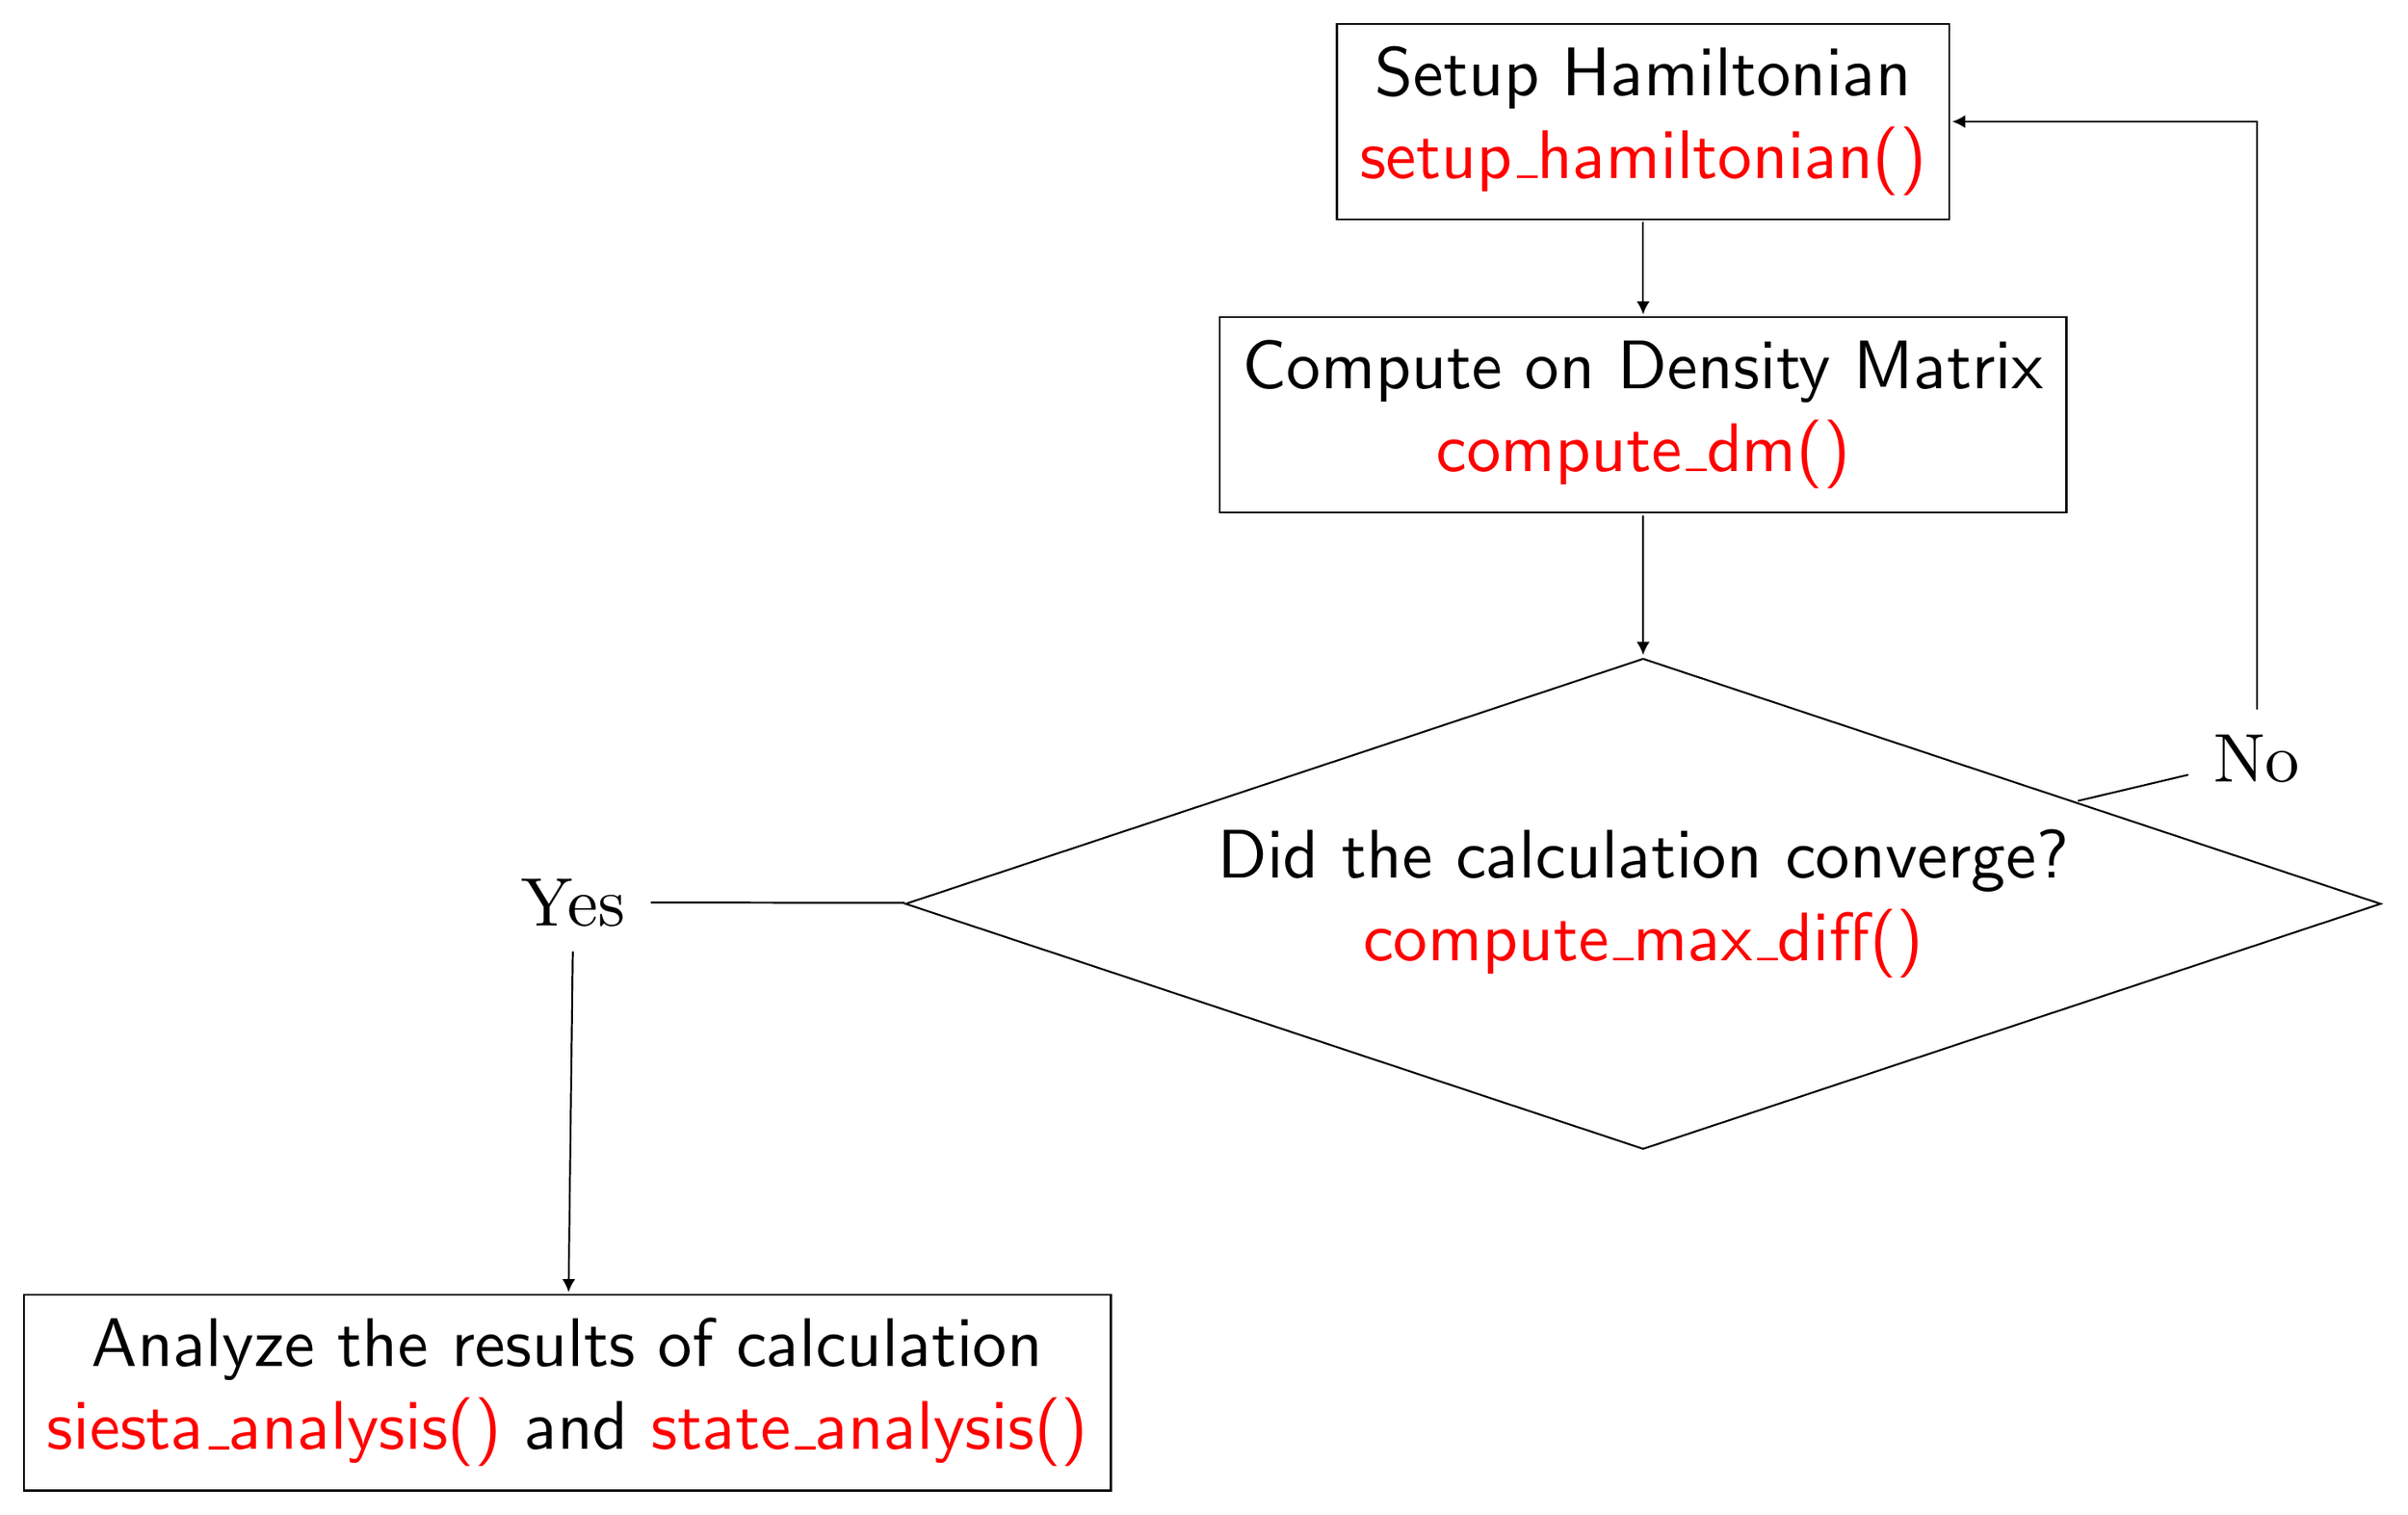
\begin{tikzpicture}[
  thick,
  scale=3.0,
  node distance=1.5cm,
  align=center,
  every node/.style={
    fill=white,
    % font=\sffamily,
    transform shape
  },]
  % nodes
  \node (setup_H)  [action]
  {Setup Hamiltonian \\ \textcolor{red}{setup\_hamiltonian()}};
  \node (compute_dm)  [action, below of=setup_H]
  {Compute on Density Matrix \\ \textcolor{red}{compute\_dm()}};
  \node (check_conv)  [test, below of=compute_dm, yshift=-1cm]
  {Did the calculation converge? \\ \textcolor{red}{compute\_max\_diff()}};
  \node (analyze)  [action, below of=check_conv, yshift=-1cm, xshift=-5.5cm]
  {Analyze the results of calculation \\
    \textcolor{red}{siesta\_analysis()} and \textcolor{red}{state\_analysis()}};
  % lines
  \draw[->] (setup_H) -- (compute_dm);
  \draw[->] (compute_dm) -- (check_conv);
  \path(check_conv.east) to node[xshift=1cm, yshift=-1cm](conv_no){No} (setup_H);
    \draw[->] (check_conv) -- (conv_no) |- (setup_H);
  \path(check_conv.west) to node[xshift=-1cm, yshift=1cm](conv_yes){Yes} (analyze);
    \draw[->] (check_conv) -- (conv_yes) -- (analyze);
\end{tikzpicture}
\end{document}
